\chapter{Проектирование модуля}

\section{Требования к разрабатываемому модулю}

\subsection{Формулировка требований}
Сформулируем ряд функциональных требований к разрабатываемому модулю. Требования должны быть составлены 
таким образом, чтобы результат их реализации удовлетворял одной из поставленных на дипломный проект задаче ---
разработанное ПО должно в значительной степени снижать сложность осуществления функционального
и нагрузочного тестирования взаимодейтсвия клиента и сервера по AMF-протоколу.

\begin{enumerate}
\item Разрабатывамый модуль должен предоставлять возможность записи действий пользователя, 
производимых с тестируемым приложением(проксирование запросов). Проксирование является важным функциоанльным
требованием, так как на этапе подготовки тестирования позволит создавать тестовый сценарий, на основе действий 
пользователя с приложением.
\item Программный модуль должен предоставлять возможность отправки AMF сообщений через http соединение по
указанному url
\item Программный модуль должен полностью поддерживать протокол AMF с целью кодирования, декодирования и замены
сообщений. Все полученные или отправленные сообщения должны предоставляться пользователю в человекочитаемом
формате.
\item Реализация программного модуля должна полностью поддерживать основные прнципы нагрузочного тестирования
имитирующего работу большого количества пользователей одновременно.
\item Разрабатываемое приложение должно интегрироваться с системами автоматической сборки проектов, такими как maven и ant
\item Возможность запуска тестов из командной строки. Данная возможность позволяет
выполнять тесты в автоматическом режиме в системах непрерывной интеграции, что
является необходимостью, особенно в тех случаях, когда над разными частями
тестируемой системы разработчики трудятся независимо и необходимо
выполнении частых автоматизированных сборок проекта для скорейшего
выявления и решения интеграционных проблем. Часто производители тестовых
фреймворков предоставляют свои продукты для проведения интеграционного тестирования, однако
зачастую они узко заточены под конкретный круг задач, поэтому нас будет интересовать
возможность запуска тестов на таких инструментах интеграции, как Jenkins и
Hudson, которые на данный момент широко распротранены и имеют множество плагинов, позволяющих
значительно расширить их существующую функциональность.
\item Кроссплатформенность. Созданная нами тестовая утилита должна работать
под управлением различных операционных систем.
\item Условия распростронения продукта. В идеале программное обеспечение должно быть
бесплатным и иметь открытый исходный код с возможность создания собственных расширений,
это является одним из основных критериев отбора, так как тестировщики и разработчики
всегда должны иметь возможность доработки и усовершенствования существующего функционала
тестового фреймворка, чтобы адаптировать его под специфику работы тестируемого ими приложения.
\end{enumerate}

\subsection{Анализ требований} 
Проанализируем сформулированные требования к разрабатываемому модулю.
Для наглядности и удобства сведём их в таблицу.

ТУТ ТАБЛИЦА

Для классификации требований были выбраны следующие критерии:

\begin{enumerate}
\item Приоритет --- критерий оценки полезности реализации требования для конечного пользователя,
важности для достижения поставленных перед проектом целей.
\item Трудоёмкость --- критерий отображает предварительную оценку сложности реализации требования,
количество привлекаемых для этого ресурсов.
\item Риск --- интегральный критерий, введением которого предпринимается попытка оценить во-первых
возможность невыполнения требования, во-вторых возможную ошибку в оценке по двум предыдущим
критериям (в первую очередь  трудоёмкости).
\end{enumerate}

Для каждого из критериев введена шкала из трёх уровней: низкий, средний, высокий.
Размерность шкалы выбрана минимальной исходя из соображений простоты и наглядности.
Так как размер проекта и количество предъявляемых к нему требований незначительны,
то таких шкал вполне достаточно для исчерпывающей классификации требований а также принятия
проектных и организационных решений.

\section{Архитектура модуля}


\begin{figure}[ht]
\center{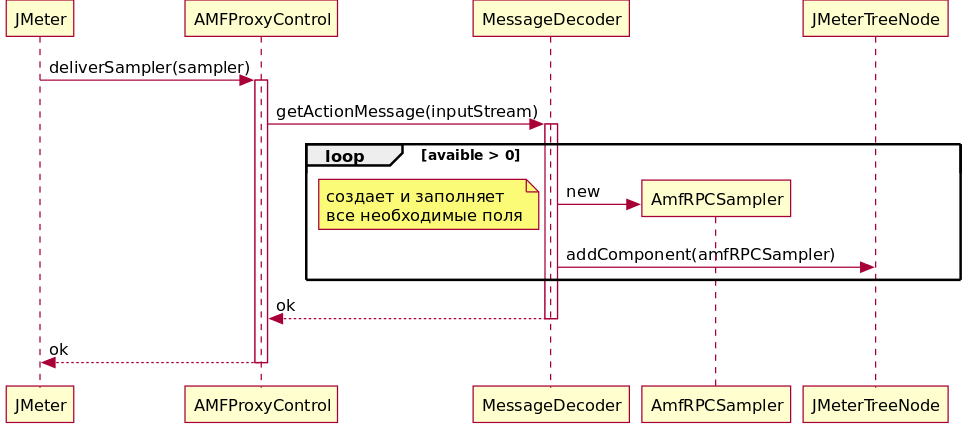
\includegraphics[height=120mm, width=120mm]{fig/development/Diagram1.png}}
\caption{Структура проекта JMeter}
\label{ris:JMeterProject.png}
\end{figure}